\paragraph{Stall Unit}

\begin{figure}[H]
    \centering
    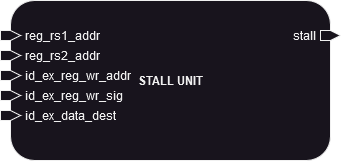
\includegraphics[width=0.5\textwidth]{design/pipelined/decode/images/stall_unit.png}
    \caption{Diagram of the Stall Unit}
    \label{fig:stall_unit}
\end{figure}

The stall unit is a small module that is used to stall the pipeline when a data dependency that cannot be resolved by forwarding is detected
which should only happen if we use the result of a load instruction in the next instruction. It is simply comparing the register addresses of the
current instruction with the register that is being written by the previous instruction. If there is a match, it looks what is the operation that is
being executed by the current instruction and if it is a load, it will stall the pipeline. \\

Signals:
\begin{enumerate}[label={\textbullet}]
    \item Input: $reg\_rs1\_addr$, This signal is representing the first register address that is being used by the current instruction.
    \item Input: $reg\_rs2\_addr$, This signal is representing the second register address that is being used by the current instruction.
    \item Input: $id\_ex\_reg\_wr\_addr$, This signal is representing the register address that is being written by the previous instruction.
    \item Input: $id\_ex\_reg\_wr\_sig$, This signal is representing if the previous instruction is written to the register file or not.
    It is used to differentiate between a load and a store.
    \item Input: $id\_ex\_data\_dest$, This signal is representing the origin of the data that is being used by the ALU in the previous instruction.
    In this case only if the previous instruction has a data dest of MEM then we need to stall the pipeline.
    \item Output: $stall$, This signal is representing if we need to stall the pipeline or not.
\end{enumerate}